%%%%%%%%%%%%%%%%%%%%%%%%%%%%%%%%%%%%%%%%%%%%%%%%%%%%%%%%%%%%%%%%%%%%%%%%%%%%%%%%%%%%5%%%%%%%%%%%%%%%
%  本文档可在安装了CTEX宏包, CTEX字体下的TEX系统运行,
%  访问http://www.ctex.org, 可以获得最新的宏包与字体安装包
%
%  请使用PDFLATEX对模板编译2次, 可得正确结果, 由于hyperref的设置中不支持DVI-PDF,
%  用LATEX编译时需要替换相应的命令, 详见相应注释.
%
% 文档是在原来李湛、何力同学的模板的基础上修改的, 主要包括以下几个地方:
%
%1.修正了原模板使用hyperref宏包中的设置, 使文档更加美观, 对设置作出了说明, 可以进一步修改
%2.修正了定理的样式, 原定理标题是黑体加粗, 现改为黑体, 原定理正文为倾斜楷体, 现改为楷体, 符合一般论文的格式
%3.对导言区的少部分命令修改, 删去了一些默认的重复的设置
%4.对模板的少部分正文进行充实
%5.对部分原来模板中的注释进行了修改, 删去了不必要的, 加入了一些中文的注释, 方便查阅
%
%  by 张越 Apr.12, 有问题请发送你的问题到:frank_melody@hotmail.com
%%%%%%%%%%%%%%%%%%%%%%%%%%%%%%%%%%%%%%%%%%%%%%%%%%%%%%%%%%%%%%%%%%%%
%%%%%%%%%%%%%%%%%%%%%%%%%%%%%%%%%%%%%%%%%%%%%%%%%%%%%%%%%%%%%%%%%%%%%%
% documentclass can be ctexart, ctexrep, ctexbook, 推荐使用模板中的CTEXREP
% cs4size - 默认的字体大? ∷?% punct - 对中文标点的位置(宽度)进行调整
% twoside - if you want to print on both side of the paper, or else you should omit this
\documentclass[notitlepage,cs4size,punct,oneside]{ctexrep}

% default paper settings, change it according to your word
\usepackage[a4paper,hmargin={2.54cm,2.54cm},vmargin={3.17cm,3.17cm}]{geometry}

\usepackage{amsmath,amssymb,amsthm}

% 公式编号的计数格式, 在章内计数
\numberwithin{equation}{chapter}

% set the abstract format, need abstract package

\usepackage[runin]{abstract}

%使用hyperref宏包, 对目录, 公式引用, 文献引用做超链接, 超链接方便电子版的阅读, 但不影响打印
% pdfborder对超链接的边框大小进行设置, 模板中默认边框大小为0
% colorlinks=true, 表示超链接对应的文字采用超链接边框的颜色, =false时保持原字体颜色
% linkcolor=blue, 设置超链接边框的颜色, 可以改为red,green等等.
% CJKbookmarks=true, 生成PDF中文书签,
% 非CTEX套装用户可能发现即便如此设置, 生成的PDF书签也是乱码, 需要用GBK2UNI.EXE解决
\usepackage[pdfborder={0 0 0},colorlinks=true,linkcolor=blue,CJKbookmarks=true]{hyperref}
\usepackage{float}
\usepackage[noend]{algpseudocode}
\usepackage{algorithmicx,algorithm}
%若要用LATEX编译, 请用下面的命令替代上述命令:
%\usepackage[dvipdfm,pdfborder={0 0 0},colorlinks=true,linkcolor=blue,CJKbookmarks=true]{hyperref}

\setlength{\absleftindent}{1.5cm} \setlength{\absrightindent}{1.5cm}
\setlength{\abstitleskip}{-\parindent}
\setlength{\absparindent}{0cm}

% Theorem style
\newtheoremstyle{mystyle}{3pt}{3pt}{\kaishu}{0cm}{\heiti}{}{1em}{}
\theoremstyle{mystyle}

\newtheorem{definition}{\hspace{2em}定义}[chapter]
% 如果没有章, 只有节, 把上面的[chapter]改成[section]
\newtheorem{theorem}[definition]{\hspace{2em}定理}
\newtheorem{axiom}[definition]{\hspace{2em}公理}
\newtheorem{lemma}[definition]{\hspace{2em}引理}
\newtheorem{proposition}[definition]{\hspace{2em}命题}
\newtheorem{corollary}[definition]{\hspace{2em}推论}
\newtheorem{remark}{\hspace{2em}注}[chapter]
%类似地定义其他“题头”. 这里“注”的编号与定义、定理等是分开的

\def\theequation{\arabic{chapter}.\arabic{equation}}
\def\thedefinition{\arabic{chapter}.\arabic{definition}.}

% title - \zihao{1} for size requirement \heiti for font family requirement
\title{{\zihao{1}\heiti{} 在推荐系统中估计曝光度}}

\author{周易\\学号:13300180065\\专业:数学与应用数学}

\date{2017年5月16日}
%%%%%%%%%%%%%%%%%%%导言区设置完毕
%%%%%%%%%%%%%%%%%%%%%%%%%%%%%%%%%%%%%%%%%%%%%%%%%%%%%%%%%%%%%%%%%%%%%
\begin{document}
%Styles for chapters/section
%若要将章标题左对齐, 用下面这个语句替换相应的设置
%\CTEXsetup[nameformat={\raggedright\zihao{3}\bfseries},%
\CTEXsetup[nameformat={\zihao{3}\heiti},%
           titleformat={\zihao{3}},%
           beforeskip={0.8cm},afterskip={1.2cm}]{chapter}
\CTEXsetup[nameformat={\zihao{4}\bfseries},%
           titleformat={\zihao{4}},%
           name={第~,~节},number={\arabic{section}},%
           beforeskip={0.4cm},afterskip={0.4cm}]{section}
\CTEXsetup[format={\zihao{-4}\bfseries},%
           titleformat={\zihao{-4}},%
           number={\arabic{section}.\arabic{subsection}.},%
           beforeskip={0.4cm},afterskip={0.4cm}]{subsection}
\CTEXoptions[abstractname={摘要:}]
\CTEXoptions[bibname={\heiti 参考文献}]

\renewcommand{\thepage}{\roman{page}}
\setcounter{page}{1}
\tableofcontents\clearpage

\maketitle\renewcommand{\thepage}{\arabic{page}}
\thispagestyle{empty}\setcounter{page}{0}
%%%  论文的页码从正文开始计数, 摘要页不显示页码
% 撰写论文的摘要
\begin{abstract}
在面对信息过载的问题的时候,推荐系统可以为用户提供个性化的推荐物品列表,因此推荐系统在电子商务、电子音乐等领域都有着广泛的应用。协同过滤是一种常用的推荐方法,通过分析用户的偏好和物品(比如商品,歌曲,游戏等)的属性,来发掘出未知的“用户-物品”关系。空缺数据是推荐系统必须面对的一个问题,传统的推荐方法\cite{WMF}将包括空缺信息在内的所有的数据都考虑进去加权处理,然而这是有失偏颇的,因为每个用户的视野和精力是有限的,有些物品根本没曝光在用户眼前,因此对应的那些空缺数据是难以反应用户偏好的。因此,一种通过概率方法估计物品曝光度的混合模型\cite{EXPOMF}被提了出来,该方法把物品曝光在用户面前与否看成模型中的一个隐变量,从而将原始的数据作了区分,更加能反映客观现实,也更具有可解释性。然而我在实践中发现该模型在一些隐式反馈数据集上表现不好,本文分析了其中的原因,并改进了该模型,从而可以处理各种类型的隐式反馈数据集,并在一些新的数据集上利用这个混合模型做了实验性的探索,进一步探究了该模型的各方面性能。
\\
\\
\\
\noindent{\heiti 关键字:} 协同过滤,概率图,混合模型,EM方法,推荐系统
\end{abstract}


\chapter{引言}

为合适的用户推荐合适的物品,在这个信息量飞速增长的时代是一个非常重要的问题。一方面,面对过于庞大和冗杂的信息库,用户节约了自己亲自去搜索和试验未知事物的时间,可以直接获得一个经过分析历史数据而得到的个性化推荐列表;另一方面,对拥有自己产品和大量用户的公司来说,更好的满足了客户需求,因此能够取得更好的商业表现,赚取更多的利润。协同过滤就是一种出色的推荐方法。
\par
具体地说,使用协同过滤的推荐系统面对的是这样一个问题:观测到一组用户和物品交互的信息,可以是评分、点击、浏览等,我们的目标是从中推断出用户的偏好,然后借助分析得到的用户偏好来为他们推荐物品。
\par
从策略上来说,协同过滤可以有两种思路。一种是“邻居方法”(neighborhood method),邻居方法专注于计算用户与用户之间、物品与物品之间的关系。比如,在电子商务中,通过计算得到商品之间的相似度之后,可以为用户推荐与他们曾经购买过的具有相似属性的物品。在电影评价估计中,通过计算得到得到用户之间的相似度之后,在估计一个用户对一部他没有看过的电影的时候,可以选取一部分和他思想相近、兴趣相投的用户,利用他们对这部电影的评价来估计该用户对这部电影的喜好。另一种是”隐向量方法”(latent factor method),这种方法和矩阵的奇异值分解有很大关系,奇异值分解在信息检索问题中被认为是一个很好的得到隐语义向量(latent semantic factors)的方法。类似的,它把得到的观测值看做一个“用户-物品”矩阵,然后将推荐看做一个矩阵的分解问题,分解得到的是一组用户向量和一组物品向量,这些向量刻画的是用户和物品的各种属性。在估计某用户是否喜欢某个物品的时候,只需要将该用户对应的向量和该物品对应的向量做点积,把这个乘积当做用户对物品的“偏好”的估计。在这篇文章使用的是“隐向量方法”。
\par
从数据性质上来说,协同过滤可以分为从显式反馈数据中推荐和从隐式反馈数据中推荐。最方便而且高质量的数据是显式反馈数据,显式反馈数据是指用户自己记录的对物品的评价。比如说豆瓣网用户对不同书籍的评分,比如Netflix利用一个大拇指朝上或朝下的按钮,对它的用户收集的在对观看过的电影和电视剧的评价。推荐系统可以通过用户反映的喜欢或者讨厌,推断出用户的偏好。但是显式反馈数据往往比较难以获取,因为他们需要用户的参与才能采集到,需要用户自己参与进对物品的评价,相对而言是一种“昂贵”的数据。另一种更加容易得到的,范围更广的数据是隐式反馈数据。隐式反馈数据,往往是用户行为的副产品,包括用户的点击、对商品的浏览、过往的购买记录和观看电视剧的总时长等。从隐式反馈中推断用户的偏好往往比从显式反馈更难,因为用户没有明确表达他们的喜欢和讨厌。
\par
隐式反馈的数据的特点决定了它们不能直接使用成熟的、被广泛研究的处理显式反馈数据的方法。隐式反馈数据的主要性质有以下:

\begin{itemize}
\item[-] \textbf{没有负面反馈.}通过观察用户的行为,我们可以推测出用户大概会喜欢某些选项,但是很难推断你到底是不是不喜欢一些选项。比如某个用户在在线音乐平台上点击了一首摇滚乐团五月天的歌曲,这个数据可以反应这个用户有可能喜欢摇滚类型的音乐或者说他就是五月天的粉丝。但你不能通过他没有点击另一首古典音乐就断定该用户不喜欢这种类型的音乐或这位音乐家。因为有可能是那位古典音乐的音乐人相对商业化成功的五月天来说影响力比较小,曝光度很小,用户根本没有发现这个音乐,所以没有点击。没有负面反馈的这个性质,导致我们必须考虑一整个“用户-数据”矩阵,包括用户的正面反馈和空白反馈,并且从看上去是“空白信息”的反馈中,发掘负面的反馈。
\item[-] \textbf{数值信息不能代表用户喜好.}在显式反馈数据中,用户明确地表达了他们的喜好,比如给非常喜欢的电视剧打五分,给不喜欢的电视剧打一分。但是在隐式反馈数据中,用户喜好不能直接从数值信息上看出来。隐式反馈数据往往代表着签到信息,购买记录,观看时长,用户行为的频率等。比如一个用户看两部电视剧《人民的名义》和《生活大爆炸》,观察到他每周花在《人民的名义》上的时间长于《生活大爆炸》。但这个信息并不能有力地证明该用户更喜欢《人民的名义》,因为也许这个用户的习惯就是每周看一集在看的剧集,但是《人民的名义》每集的长度就是长于《生活大爆炸》。但是相对的,我们可以说,我们对这个用户行为更有“信心”,意思是数值上大的用户行为更可能是一种稳定的可靠的用户行为,而不是用户突发其想产生的行为。
\end{itemize}

\par
为了处理上述的问题,加权的矩阵分解方法\cite{WMF}(Weighted Matrix Factorization, 简写为WMF)引入了启发式的想法,给予用户的各种行为不同的信心(Confidence),对那些“空白信息”给予很低的信心,并把用户行为看做一个二值化的决定(即非0即1的数据),从而把问题处理成一个回归的问题。但是这种方法是存在问题的是它把所有的数据都以同一种模式处理。
\par
WMF借鉴了处理显式反馈数据的方法,但是过高地估计了没有点击的物品的权重,因为,可以想象的是,面对如今网络上越来越丰富的物品选项,对于绝大多数用户没有点击的数据来说,用户都是因为没有看到他们才没有点击,只有其中一小部分是因为不喜欢才没有点击。于是另一种想法\cite{EXPOMF}是摒弃之前的启发式的观点,采取直接的概率手段,对物品是否曝光在用户面前进行了建模,同时继承了之前的把用户行为二值化的想法。把因为用户不喜欢一个物品而没有点击和用户因为没有发现这个物品而没有点击区分了开来,因此建立了一个混合模型,称为模拟曝光率的矩阵分解方法(Exposure Matrix Factorization, 简写为 ExpoMF)。

\par
ExpoMF更能反映现实的情况,实验的效果也更加优异。只是,有一个问题在于虽然原方法在处理二值化的数据,比如签到、购买等数据的时候比较优异,但在反映表示频率,点击次数,时长的这种含有“用户行为强烈程度”的隐性数据的时候效果不够理想,于是我将\cite{WMF}中的信心概念重新引入到ExpoMF中,因为原来的启发式想法并不是完全一无是处的,信心虽然不应该直接用作为回归的权重,但数值的相对大小可以帮助我们进行“曝光度”的建模,补充了ExpoMF,使得它可以处理新的数据类型。
\par
我将ExpoMF模型处理了来自在线音乐平台的音乐的点击数据,电影评价网站的的电影观看数据和在线游戏公司的游戏购买数据。在实验中,ExpoMF在衡量推荐效果的各个标准下,都超过了目前为止最主流的方法——WMF\cite{WMF}。
\par
本文接下来的部分按以下顺序展开:在第二章背景知识中回顾采用隐向量方法的协同过滤模型,在第三章中描述一整套ExpoMF模型。在第四章中,详细地描述了在各种数据集上的实验过程、评价体系和实验结果。在第五章中给出了结论。



\chapter{背景知识}
在这一章中,第一节介绍了隐向量方法以及它是如何处理显式反馈数据的。第二节介绍了如何通过类比,处理隐式反馈数据。第三节介绍了,如何从概率的角度来看待隐向量方法。

\section{协同过滤的隐向量方法}
隐向量方法把推荐系统内的所有的用户(user)和物品(item)映射到一个$K$维的实向量空间上:每个物品对应于一个向量,这个向量叫做物品的隐向量$\beta_i\in R^K$,这个向量的每个坐标反映一个属性维度。每个用户对应于一个向量$\theta_u\in R^K$,这个向量叫做用户的隐向量,刻画了用户在各个属性上的感兴趣的程度。使用相应的两个向量的内积$\theta_u^T\beta_i$去刻画用户$u$和物品$i$的相关程度——用户对物品的总体的感兴趣的程度。
\par
我们把观察到的数据记为矩阵$R$,矩阵中每个数据为$r_{ui}$。每个数据条目记录的相应的用户行为信息。上述的想法可以描述$$\hat{r_{ui}}=\theta_u^T\beta_i$$
\par
因为,观察到的数据矩阵是非常稀疏的,有很多空缺值。早期的方法是去填补空缺值,去做矩阵的分解,然而这样做的代价非常昂贵,以矩阵的奇异值分解为例,SVD分解的时间复杂度是三次方级别的,当数据量变大的时候,计算代价会变得非常大。早期的方法面对的另一个问题是,面对如此稀疏的数据真的值得我们去填补空缺值吗?
\par
于是,当Netflix——美国的一个在线影视公司——举办\href{http://www.netflixprize.com/}{Netflix Prize}比赛的时候,给出一个巨大的数据集,让全世界的参赛者帮他们解决预测电视电影评分预测的问题的时候,早期的方法就陷入了困境。于是参赛者想出了直接在观察到的数据集上进行隐向量的学习,同时引入正则化项避免过拟合的问题,这个想法成为后来的主流方法。从而,原问题被理解成了一个在观察值上训练用户隐向量和物品隐向量的回归问题。
\par
对于一个显性反馈数据集的带正则化项的最小二次误差模型如下:
\begin{equation}\label{ExplicitMF}
\min_{\theta,\beta}\sum_{u,i\in K}(r_{ui}-\theta_u^T\beta_i)^2+\lambda(\sum_u||\theta_u||^2+\sum_i||\beta_i||^2)
\end{equation}
\par
这里$K$是指被观察到的、已经被记录的数据对的集合(比如所有的用户评分)。

\section{处理隐式反馈数据的隐向量方法}\label{introToWMF}
当面对隐性反馈数据的时候,情况变得不再相同。为了克服隐性反馈数据的特性,加权的矩阵分解方法(Weighted Matrix Factorization)\cite{WMF}被提出,这也是目前最主流、效果优秀的方法。这个模型采用的是简单的启发式想法,给予不同的数据点不同信心,作为回归的系数。

\par
WMF首先将原始的数据二值化:
$$ y_{ui}=\left\{
\begin{aligned}
0, \qquad if (r_{ui}=0) \\
1, \qquad if (r_{ui}>0)
\end{aligned}
\right.
$$
\par
然后根据不同的原始数据,给每个数据点不同的信心(Confidence)作为回归的权重。具体的信心函数因数据的种类而异,原始数据的值越大,我们相对的确信用户对喜欢那个物品的信心就越大。举个例子,常见的信心函数可以选择为线性函数或对数函数:
\begin{equation}\nonumber
c_{ui}=1+\alpha y_{ui}\qquad or \qquad
c_{ui}=1+\alpha log(1+y_{ui}/\epsilon)
\end{equation}
\par
和处理显式反馈的方法做类比,WMF把处理隐式反馈数据,归结为如下的回归问题:
\begin{equation}\label{ImplicitMF}
\min_{\theta,\beta}\sum_{(u,i)}c_{ui}(y_{ui}-\theta_u^T\beta_i)^2+\lambda(\sum_u||\theta_u||^2+\sum_i||\beta_i||^2)
\end{equation}



\section{隐向量分解的概率解释}
用隐向量分解矩阵,也可以从概率的角度出发,得到的结论和之前一致,但是是一种不同的诠释,相应的方法称为概率矩阵分解(Probabilistic matrix factorization,简写为PMF)\cite{PMF}
\par
概率矩阵分解,从生成数据的模型的角度看,假设用户向量$\theta_u$和物品向量$\beta_i$两个特定的分布中生成,分别代表着用户的偏好和物品的属性。然后,观察值在从一个期望为$\theta_u^T\beta_i$的分布中生成。具体地说,一个正态分布的矩阵分解可以写成:
\begin{eqnarray*}
&&\theta_u  \sim  \mathcal{N}(0,\lambda_\theta^{-1} I_K)\\
&&\beta_i  \sim  \mathcal{N}(0,\lambda_\beta^{-1} I_K)\\
&&r_{ui} \sim \mathcal{N}(\theta_u^T\beta_i,\lambda_r^{-1} )
\end{eqnarray*}

\par
由以上的模型,我们可以计算观察值的出现的概率,针对本章第一节的显式反馈数据,我们有:
\begin{eqnarray*}
\prod _{(u,i)\in K} P(r_{ui})&=& \prod _{(u,i)\in K} P(r_{ui}|\theta_u,\beta_i)P(\theta_u)P(\beta_i)\\
&\sim& \prod _{(u,i)\in K}e^{-\frac{\lambda_r}{2}(r_{ui}-\theta_u^T\beta_i)^2}e^{-\frac{\lambda_\theta}{2}\theta_u^T\theta_u}e^{-\frac{\lambda_\beta}{2}\beta_i^T\beta_i}
\end{eqnarray*}

\par
采用最大似然估计的想法,最大化上述概率,我们就可以得到:
\begin{eqnarray*}
\max_{\theta,\beta}\prod _{(u,i)\in K} P(r_{ui})&=& \max_{\theta,\beta}\quad log\prod _{(u,i)\in K} P(r_{ui})\\
&=& \min_{\theta,\beta}\quad \lambda_r(r_{ui}-\theta_u^T\beta_i)^2+\lambda_\theta||\theta_u||^2+\lambda_\beta||\beta_i||^2
\end{eqnarray*}

这里$||.||$是2-范数。

\par 
如果我们取$\lambda_\theta=\lambda_\beta$,那么我们就得到了公式(\ref{ExplicitMF})。
\par
同理,针对隐性反馈数据,PMF可以改写成:
\begin{eqnarray*}
&&y_{ui} \sim \mathcal{N}(\theta_u^T\beta_i,c_{ui}^{-1} )
\end{eqnarray*}

\par
这里,第二节中描述的“信心”。类似地,利用最大似然估计去估计参数,我们可以得到公式(\ref{ImplicitMF})。



\chapter{ExpoMF模型}
在这章中给出ExpoMF的描述。第一节给出模型的介绍,第二节给出估计曝光度的方法,第三节给出模型的推断算法。
\section{模型描述}
在推荐系统中,每个观测数据,都可以用用户$u=1,2,3..U$和物品$i=1,2,3…I$的组合来标记。
\par
ExpoMF是用于处理隐式反馈数据。隐式反馈数据也有不同种类,如果是反应点击次数,观看时间长短的隐式反馈数据,在这里就可以用$r_{ui}$表示。按照处理隐式反馈数据的方法,将其二值化(0或1),沿用之前的记号,记为$y_{ui}$,另一种本身就是0-1型的隐式反馈数据,比如是否观看某电影的记录,电子游戏的购买记录等,就直接记为$y_{ui}$。
\par
接下来,对于每个组合$(u,i)$,我们引入一个隐变量$z_{ui}$,用这个变量去描述,用户$u$是否暴露在物品$i$面前:若$z_{ui}=1$,则代表用户$u$已经看到了物品$i$,之后的用户行为,就可以由他的偏好和物品的属性解释,和标准的方法类似的,用一个K维向量$\theta_u$来描述用户u的偏好,用一个向量$K$维向量$\beta_i$来量化物品$i$的属性,用它们的内积估计这个用户行为的程度;若$z_{ui}=0$,则代表用户根本没有看到物品$i$,因此后面他不应该会对物品做任何动作(点击,购买等)。
\par
根据物品是否暴露在用户面前,我们得到以下混合模型:
\begin{eqnarray*}
&&\theta_u  \sim  \mathcal{N}(0,\lambda_\theta^{-1} I_K)\\
&&\beta_i  \sim  \mathcal{N}(0,\lambda_\beta^{-1} I_K)\\
&&z_{ui} \sim Bernoulli(\mu_{ui})\\
&&y_{ui}|z_{ui}=1 \sim \mathcal{N}(\theta_u^T\beta_i,\lambda_y^{-1} I_K)\\
&&y_{ui}|z_{ui}=0 \sim \delta_0
\end{eqnarray*}

这里$\delta_0$,表示$P(y_{ui}=0|z_{ui}=0)=1$,而$\mu_{ui}$表示我们对该物品是否会暴露在用户面前的一个先验估计,其余符号均沿用之前的含义。上述模型的概率图表示在图~(\ref{figure:ExpoMF})(a)中给出。


\begin{figure}[h]
 \centering
 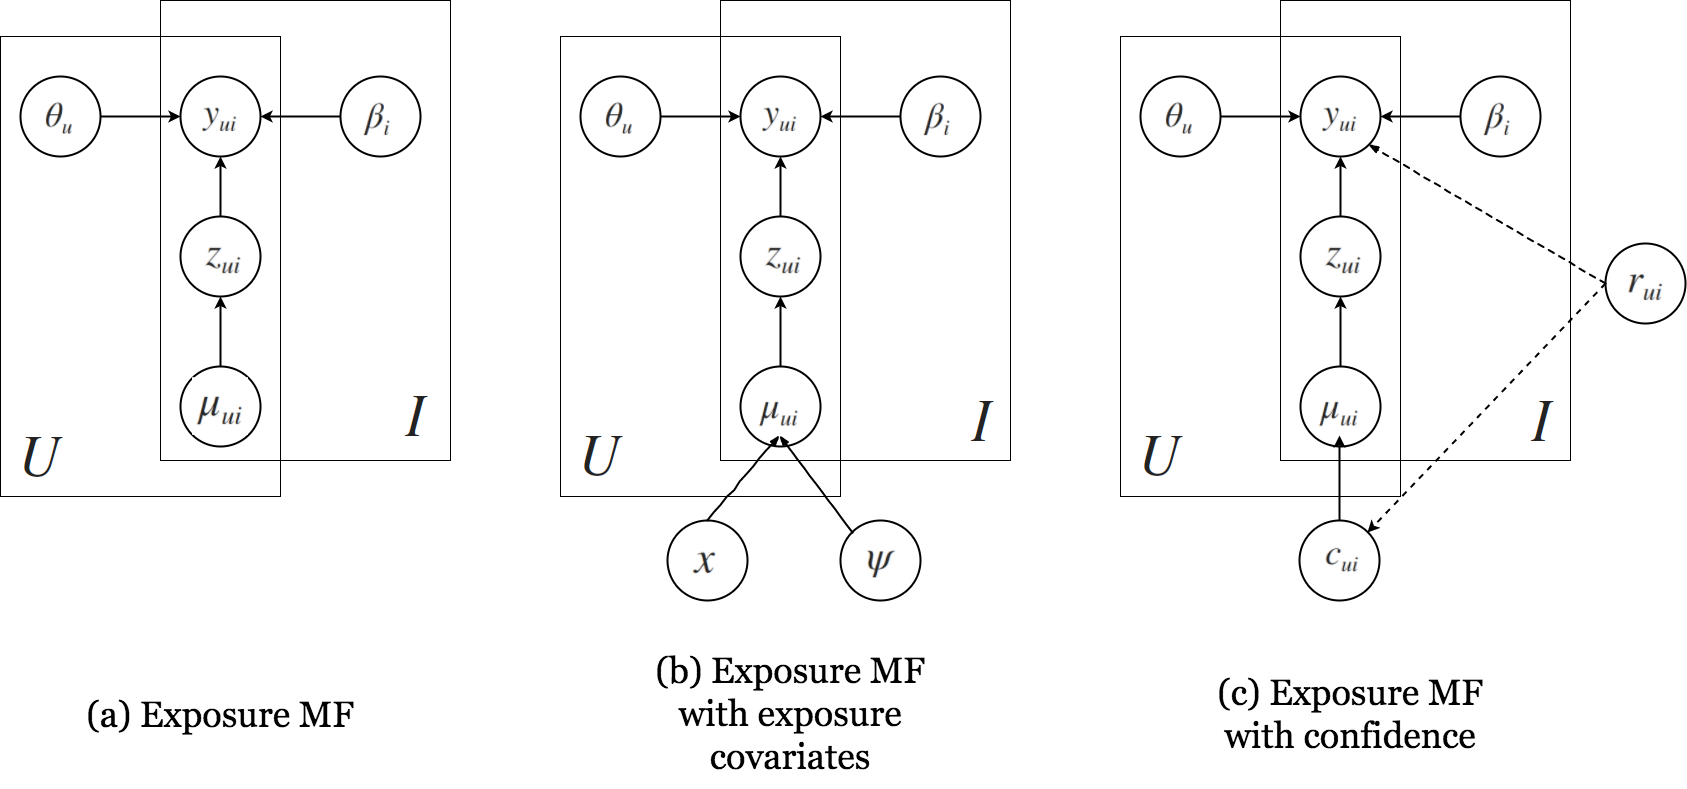
\includegraphics[width=\textwidth]{./equations/graph1.png}
 \caption{ExpoMF的概率图表示。一条带箭头的、从a到b的实线段表示,在模型中b的生成依赖于a。一条带箭头的、从a到b的虚线段表示,在模型中b是a数据处理后的结果}
 \label{figure:ExpoMF}
\end{figure}

\par
在开始计算这个ExpoMF模型之前,我们手上的数据是一个用户-物品兴趣矩阵$Y=\{y_{ui}\}$,每个$y_{ui}$标记着用户u是否对物品i感兴趣,0代表不感兴趣,1代表感兴趣。ExpoMF区别于其他矩阵分解的方法的地方在于,它有一个暴露矩阵$Z=\{z_{ui}\}$,运用这个暴露矩阵$Z$把兴趣矩阵$Y$的分解看做一个混合模型。这个两个矩阵之间是有联系的。如果$y_{ui}=1$,那么$z_{ui}=1$,因为你如果对一物品表现出了兴趣(发生了购买、点击),那么这个物品一定已经被你观察到了。但如果$y_{ui}=0$,那么$z_{ui}$对我们来说是未知的,这也是我们需要去建立模型模拟的关键点。从实践的角度说,因为兴趣矩阵$Y$往往是非常稀疏的,所以绝大多数的$z_{ui}$都是未知的.

\par
ExpoMF模型推导出的概率公式如下:
\begin{equation}\label{hybrid}
P(z_{ ui },y_{ ui }|\theta _{ u },\beta _{ i },\mu _{ ui },\lambda _{ y }^{ -1 })=[\mu _{ ui }N(y_{ ui }|\theta _{ u }^{ T }\beta _{ i },\lambda _{ y }^{ -1 })]^{ z_{ ui } }[(1-\mu _{ ui })\delta _{ 0 }(y_{ ui })]^{ (1-z_{ ui }) }
\end{equation}

\par
和WMF类似,ExpoMF也会选择性地降低”空缺值“对模型的影响,但是区别在于不是利用方差项来降低影响,而是通过判断是否该物品是否暴露在用户面前,调整模型的混合程度,来降低”空缺值“的影响。
\par
公式~(\ref{hybrid})显示这是一个混合模型,如果把所有的$z_{ui}$都固定为1,那么我们重新发现了标准的矩阵分解方法。
\par
在进行更进一步的描述之前,先来看看为什么这个模型对隐式反馈数据起作用。对公式~(\ref{hybrid})取对数函数后,我们有:
\begin{equation}\label{log-hybrid}
logP(z_{ ui },y_{ ui }|\theta _{ u },\beta _{ i },\mu _{ ui },\lambda _{ y }^{ -1 })=logBernoulli(z_{ui}|\mu_{ui})+z_{ui}logN(y_{ ui }|\theta _{ u }^{ T }\beta _{ i },\lambda _{ y }^{ -1 })+(1-z_{ui})log\delta _{ 0 }(y_{ ui })
\end{equation}

\par
设想一个情景,当一个用户$u$对物品$i$有很大的偏好的时候($\theta_u^T\beta_i$比较大),但没有发生用户行为($y_{ui}=0$),那么我们可以发现公式(\ref{log-hybrid})右边的第二项会变得很非常小,甚至是负数,这会成为一个惩罚项,迫使$z_{ui}$选择一个非常小的值。换句话说,这个模型认为:如果你喜欢一个东西,但我们发现你没有去点击它,那么很有可能是因为你没看见它。

\section{为曝光度建模}

之前在第一节中的讨论没有涉及到如何选择和学习先验估计$\mu_{ui}$。接下来分析如何估计$\mu_{ui}$。
\par
估计曝光度的方法当然是和你目前掌握了什么信息有关。下面根据掌握信息的不同,提出三种可能的方法。前两种来自\cite{EXPOMF},第三种由本文提出。


\begin{itemize}
\item[-] \textbf{Per-Item $\mu_i$:}当没有任何外部信息的时候,最简单的估计方法,就是统计每个物品的在所有用户面前的曝光度,作为$\mu_{ui}$
\item[-] \textbf{Exposure covariates:}当推荐带有文本或者地理信息的物品时候,可以首先将文本信息通过自然语言处理处理成$L$维的向量,每个维度表示文本内容的主题,或者将地理信息进行聚类成$L$个分类,得到一个包含分类信息的$L$维向量。值得注意的是,这里的$L$维和隐向量方法的$L$维没有任何关系,不一定要取相同的值。把这个向量记做$x_i$,在两种情形下,$x_i$都应该被规范到单位长度。在模型中,我们对如下函数进行学习:$$\mu_{ui}=\sigma(\psi_u^Tx_i)$$这里,$\psi_u$是模型需要学习的关于$x_i$的协变量。$\sigma$是sigmoid函数。从可解释性的角度来说,$\psi_u$可以被理解为用户平常花在各种主题的文本中的时间或者出现在各个地理位置的频率。
\item[-] \textbf{Confidence-Per-Item $\mu_i$:}当推荐用户行为中带有频率和或者反映时间长短的物品的信息的时候,直接套用\textbf{Per-Item $\mu_i$}效果会不够理想。原因是忽视了用户数据中反映用户行为的强烈程度的原始信息,这导致对$\mu_{i}$的估计不够准确。比如,对于音乐点击数据来说,一个频繁点击某首歌的用户行为,显然不应该和点击过一次某首歌的用户行为划上等号。为了量化不同的用户行为,重新引入\cite{WMF}中的“信心函数”是有必要的,把用户行为的信心作为权重,计算物品的在所有用户面前的曝光度,作为$\mu_i$。

\end{itemize}

\section{模型推断}
因为ExpoMF模型是一个带有隐变量混合模型,我们使用处理带有隐变量的模型的成熟方法——EM方法(expectation-maximization)去估计本模型的参数。EM方法可以被理解成两步,先在已有的模型中估计隐变量的值(E-Step),然后,在知道隐变量之后,利用最大似然估计,估计模型的参数(M-step)。
\subsection{用EM方法推断隐向量$\theta_u,\beta_i$}
\begin{itemize}
\item[-] \textbf{E-step:}这一步,需要估计的是暴露矩阵$Z$中的值的期望值。首先对于$y_{ui}=0$的数据,我们有:
	\begin{eqnarray*}
	E(z_{ui}|y_{ui}=0,\theta_u,\beta_i,\mu_{ui})&=& P(z_{ui}=1|y_{ui}=0,\theta_u,\beta_i,\mu_{ui})\\
	&=& \frac{P(z_{ui}=1,y_{ui}=0|\theta_u,\beta_i,\mu_{ui})}{P(y_{ui}=0|\theta_u,\beta_i,\mu_{ui})}\\
	&=& \frac{P(y_{ui}=0|z_{ui}=1,\theta_u,\beta_i,\mu_{ui})P(z_{ui}=1)}{\sum_{z_{ui}}P(y_{ui}=0|z_{ui},\theta_u,\beta_i,\mu_{ui})P(z_{ui})}\\
	&=& \frac{\mu_{ui}\mathcal{N}(0|\theta_u,\beta_i,\lambda_y^{-1})}{\mu_{ui}\mathcal{N}(0|\theta_u,\beta_i,\lambda_y^{-1})+(1-\mu_{ui})}
	\end{eqnarray*}\\
	然后,对于的$y_{ui}=1$的数据,这数据本身就意味着$$E(z_{ui}|y_{ui}=1,\theta_u,\beta_i,\mu_{ui})=1$$为了统一记号,我们记隐变量在E-step得到的期望记为$\hat{z}_{ui}$。
	于是我们有公式:

	\begin{equation}\label{updateZ}
	\hat{z}_{ui}=\left\{
	\begin{aligned}
	\frac{\mu_{ui}\mathcal{N}(0|\theta_u,\beta_i,\lambda_y^{-1})}{\mu_{ui}\mathcal{N}(0|\theta_u,\beta_i,\lambda_y^{-1})+(1-\mu_{ui})}, \qquad if (y_{ui}=0) \\
	1, \qquad if (y_{ui}=1)
	\end{aligned}
	\right.
	\end{equation}

\item[-] \textbf{M-step:}在这一步中需要在当前隐变量的期望值和观察值下,求参数的最优估计。我们这里要优化的参数是所有的隐向量$\theta_u,\beta_i$。换句话说,就是求解下述优化问题:
	$$\max_{\theta,\beta}\prod_{(u,i)}P(y_{ui},\hat{z}_{ui})=\max_{\theta,\beta}\prod_{(u,i)}P(y_{ui},\hat{z}_{ui}|\theta_u,\beta_i)P(\theta_u)P(\beta_i)$$
	取对数,得到对数似然函数$\mathcal{L}$,对$\mathcal{L}$求导,就可以得到:
	\begin{eqnarray}
	\theta _{ u } &\leftarrow& (\lambda _{ y }\sum _{ i } \hat { z}_{ ui }  \beta _{ i }\beta _{ i }^{ T }+\lambda _{ \theta  }I_{ K })^{ -1 }(\sum _{ i } \lambda _{ y }\hat { z}_{ ui }  y_{ ui }\beta _{ i })\label{updateTheta}\\
	\beta _{ i }  &\leftarrow& (\lambda _{ y }\sum _{ u } \hat { z}_{ ui }  \theta _{ u }\theta _{ u }^{ T }+\lambda _{ \beta  }I_{ K })^{ -1 }(\sum _{ u } \lambda _{ y }\hat { z}_{ ui }  y_{ ui }\theta_{ u })\label{updateBeta}
	\end{eqnarray}
\end{itemize}


\subsection{对先验估计$\mu_{ui}$的推断}
\begin{itemize}
\item[-] \textbf{Update for Per-Item $\mu_i$:}计算每个物品的在所有用户面前的平均的曝光度,作为$\mu_{ui}$的估计,也就是说:
		\begin{eqnarray}
		\mu_{ui}=\frac{\sum_{u}\hat{z}_{ui}}{U}\label{updatePerItem}
		\end{eqnarray}
		这个更新公式,也可以从最大化对数似然函数$\mathcal{L}$得出。
\item[-] \textbf{Update for Exposure covariates:}令$\mu_{ui}=\sigma(\psi_u^Tx_i)$,这里$x_i$是预处理(自然语言处理、聚类算法等)得到的向量。通过最大化对数似然函数,可以优化$\psi_u$的选择,从而更准确地估计$\mu_{ui}$。更新公式如下:
		\begin{eqnarray}
		\psi_{u}^{new}\leftarrow\psi_{u}+\gamma \bigtriangledown \mathcal{L} \label{updatePsi}
		\end{eqnarray}
		这里,$\bigtriangledown\mathcal{L}=\frac{1}{I} \sum_i (\hat{z}_{ui}-\sigma(\psi_u^Tx_i))x_i$,$\gamma$是学习率。
		每次更新完$\psi_u$之后,然后重新计算曝光率:
		\begin{eqnarray}
		\mu_{ui}=\sigma(x_i^T\psi_{u}^{new})\label{updateMuui}
		\end{eqnarray}


		

\item[-] \textbf{Update for Confidence-Per-Item $\mu_i$:}根据我们对用户行为的不同“信心”和模型目前估计的曝光度,估计$\mu_i$,即:
对于有原始“频率、时长”信息的隐性数据,根据我们对于用户行为的信心不同,计算每个物品的在所有用户面前的平均的曝光度,作为$\mu_{ui}$的估计,也就是说:
		\begin{eqnarray}
		\mu_{ui}=\frac{\sum_{u}c_{ui}\hat{z}_{ui}}{\sum_{u}c_{ui}}\label{updateConfidencePerItem}
		\end{eqnarray}

\end{itemize}

\subsection{推断算法的总结}
将前两节的讨论整理起来,可以得到如下的推断算法。

\begin{algorithm}[H]
\caption{Inference for ExpoMF} 
\hspace*{0.02in} {\bf Input:} 
binarized matrix Y,exposure covariates $x_{1:I}$(optional), raw matrix R(optional)\\
\hspace*{0.02in} {\bf Random initialization:} 
user factors $\theta_{1:U}$,user factors $\beta_{1:I}$,exposure priors $\mu_{i}$(for Per-Item and Confidence-Per-Item model),
OR exposure parameters $\psi_{1:U}$(for exposure covariates model)\\
\hspace*{0.02in} {\bf Preprocess(optional):}
Calculate confidence matrix C from raw matrix R 
\begin{algorithmic}[1]
%\State some description % \State 后写一般语句

\While{performance on validation set increase} % While语句,需要和EndWhile对应
  \State Compute expected exposure matrix Z(Equation~\ref{updateZ})
	\State Update user factors $\theta_{1:U}$(Equation~\ref{updateTheta})
	\State Update item factors $\beta_{1:I}$(Equation~\ref{updateBeta})
	\State for ExpoMF: Update priors $\mu_i$(Equation ~\ref{updatePerItem})
	\State for ExpoMF with covariates: Update covariates $\psi_u$(Equation ~\ref{updatePsi}) and recaculate priors $\mu_{ui}$(Equation ~\ref{updateMuui})
	\State for ExpoMF with confidence: Update priors $\mu_i$(Equation ~\ref{updateConfidencePerItem})

\EndWhile

\end{algorithmic}
\end{algorithm}

\section{预测}
作为一个推荐系统,我们通过给指定的用户推荐一个物品列表,通过评价这个推荐列表的好坏来评判推荐算法的好坏。
ExpoMF可以用两种方式来生成对用户$u$的推荐物品的一个推荐列表。
\begin{itemize}

\item[1] \textbf{ranked by: $\theta_u^T\beta_i$ :}和传统的MF方法类似,这个推荐方法,根据从推断算法中挖掘的用户兴趣和物品属性,找到最能满足用户口味的、感兴趣的物品。


		

\item[2] \textbf{ranked by $\mu_{ui}\theta_u^T\beta_i$ :}这个推荐方法,相当于计算了$E_y[y_{ui}|\theta_u,\beta_i]$,根据这个值来作为推荐的依据。

\end{itemize}





\chapter{实验}

在本章中,我在三个现实世界的真实数据集上,测试了ExpoMF的性能。同时通过实验的探索\footnote{重现本实验的代码可以在https://github.com/cool-pot/expo-mf-with-confidence获取},进一步研究了ExpoMF的特性。实验的结论如下:
\begin{itemize}
	\item[-] ExpoMF在这三个代表了音乐点击、游戏购买、电影观看的现实数据集合上的表现都要优秀于现在最主流的处理隐式反馈数据的方法WMF\cite{WMF}。
	\item[-] 在观察到推荐系统中的“用户行为强烈程度”信息的时候,之间使用直接的ExpoMF效果会不够好,但使用ExpoMF with confidence之后,情况会得到改善,在同等原始信息的状况下,表现优于WMF\cite{WMF}。
	\item[-] 在观察到推荐系统中的“文本、地理”信息的时候,使用ExpoMF with covariates 效果会略微好于基本的ExpoMF、好于WMF。同时,另一个好处是能够挖掘到很多关于用户的信息。

\end{itemize}

\section{数据集}
在实验中,三个数据集被利用到,分别来自不同的领域:1)音乐点击数据\footnote{https://labrosa.ee.columbia.edu/millionsong/tasteprofile},使用的是taste profile subset(TPS)来自 million song dataset\cite{MSD},记录的数据是用户对于歌曲的点击次数。这个数据集在\cite{EXPOMF}中也被利用到,但是对比的是二值化之后,ExpoMF和WMF的对比。2)游戏购买数据\footnote{https://www.kaggle.com/tamber/steam-video-games},来自kaggle数据集,记录了Steam游戏平台上对游戏的购买与否以及游戏时间。 3)电影观看数据\footnote{https://grouplens.org/datasets/movielens/},记录了用户对电影的打分,来自Movielens\cite{MLS},准确地说这是一个显式反馈数据集,但这里我们将其处理成隐式反馈数据,把每次打分当做一次观看。
\begin{itemize}
	\item[-] \textbf{Taste Profile Subset:}记录了“用户-歌曲”的点击次数,这份数据是由智能音乐公司Echo Nest收集的。在数据预处理中,为了避免矩阵出现空行或空列,我筛选了,歌曲点击数超过50、点击歌曲数超过20的用户对应的数据才会被考虑进来。同时,经过筛选的数据集仍然十分庞大,由于实验机器性能的限制,只能从中随机抽取一部分子集进行实验。
	\item[-] \textbf{Steam Game Purchase Record:} 这份数据由在线游戏公司Steam在网上公开的信息收集而来,记录了用户对游戏够买与否的数据和用户在游戏上投入了多少时间的数据。由于游戏时间的数据很不全,这里只考虑使用游戏购买的这部分数据。同样的,为了避免矩阵出现空行或空列,我筛选了,游戏购买数超过20的用户和被购买次数超过20的游戏。
	\item[-] \textbf{Movielens:} 这份数据是由GroupLens Research 从 the MovieLens web site\footnote{http://movielens.org}收集并公布的。记录了“用户-电影”的评价,每一份评价,我都对它进行了二值化,也就是说,只要打分,就认为这个用户对这部电影观看过,从而得到了一份“用户-电影”的观看记录。这本身就是一份相对来说比较稠密的数据了。从数据上看,GroupLens Research挑选的都是积极参与评价的网络用户。但是,同样的,为了避免矩阵出现空行或空列,我筛选了,观看电影数超过50的用户和被观看看数超过100的电影,留下了其中大约90\%的数据进行实验。

\end{itemize}

\begin{table}[htbp]\centering
\begin{tabular}{llll}
\hline\hline
Dataset             & TPS           & Steam     & Movielens \\
\hline
描述   				& 歌曲点击        & 游戏购买       & 电影观看      \\
原始数据中User数目     & 1,019,318     & 12,393        & 6,040       \\
原始数据中Item数目     & 384,546       & 5,155         & 3,900       \\
原始数据中数据条目      & 48,373,586    & 129,511       & 1,000,209       \\
预处理后User数目       & 1,013         & 1,269         & 4,200      \\
预处理后Item数目       & 400           & 1,197         & 2,019      \\
预处理后数据条目        & 34,147        & 75,527        & 883,466       \\
预处理后数据密度		 & 8.427\%       & 4.972\%       & 10.418\%     \\
\hline
\end{tabular}
\caption{实验数据集}\label{tab:dataset}
\end{table}

\par
关于这三个数据集的数值上的描述可以参考表\ref{tab:dataset}。总的来说,本文在较小规模的数据集(TPS和Steam)和中等规模的数据集(Movielens)进行了ExpoMF的实验,更大规模的数据集上的实验结果可以参考\cite{EXPOMF}。

\section{初步}


\subsection{实验思路}
在拿到预处理之后的数据之后,把数据按照70/20/10的标准分成训练集(train data),测试集(test data)和验证集(validation data)。

实验的思路是在训练集上的训练,以在验证集的表现作为是否可以停止训练的依据。最后评价算法的表现的时候,在测试集上进行测试。

\subsection{参照}
作为实验结果的参照,我使用了目前主流的处理隐式反馈数据的方法——WMF\cite{WMF}作为实验结果的参照。关于WMF的简洁的描述也可以参考第二章第\ref{introToWMF}节。

\subsection{评价标准}
为了评价一个推荐算法的好坏,使用这个推荐算法,给每个用户推荐一个列表。根据这些推荐列表在测试集上的平均推荐准确程度来评价这个算法的优异程度。

本文采取的评价标准如下:

\begin{itemize}
	\item[-] \textbf{Recall@k} 对每一个用户$u$计算召回率:
	$$Recall@k=\frac{\#\{i|Rank(u,i)\leq k , i\in y_u^{test}\}}{min(\#y_{u}^{test},k)}$$
	这里,$y_u^{test}$就是用户u的测试集。\#代表这个集合的计数。Recall@k反映的是推荐列表的召回率,描述了用户真正喜欢的物品中有多大的比例被推荐到。
	\item[-] \textbf{MAP@k} 对于每一个用户$u$计算平均准确率(Average Precision):
	$$AP@k=\sum_{n=1}^k\frac{Precison@n}{min(n,\#y_{u}^{test})}$$
	这里Precision@n是指推荐列表中前n个项目中,用户真正感兴趣的比例,成为准确率。
	然后,对所有的用户的AP取平均值。得到MAP@k。由计算公式可以看出,MAP@k值反映的是推荐列表的准确率,推荐列表的的项目的位置在越前面,那么影响越大。
	\item[-] \textbf{NDCG@k} 同样是用来衡量推荐列表的排名的好坏,NDCG(Normalized Discounted Cumulative Gain)采用log函数作为权重。首先对于每个用户$u$计算DCG:
	$$DCG@k=\sum_{i=1}^k\frac{2^{rel_i}-1}{log_2(i+1)}$$,这里$rel_i$取值为1若$i\in y_u^{test}$,否则为0。而IDCG@k则是DCG@k的理想情况,是一个规范系数,保证了NDCG在0和1之间:$$NDCG@k=\frac{DCG@k}{IDCG@k}$$
\end{itemize}

\section{在Steam数据上测试 ExpoMF with Per-Item}
首先在Steam游戏购买数据集上,验证ExpoMF的性能。这份数据包含了1269个用户在1197个游戏上的购买记录。对于这份数据的直观认识可以参考图\ref{figure:steam},该图描述了用户购买数和游戏被购买数量的分布。

\begin{figure}[h]
 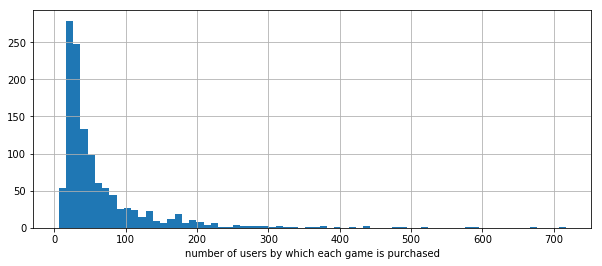
\includegraphics[width=\textwidth]{./results/game_play_by.png}
 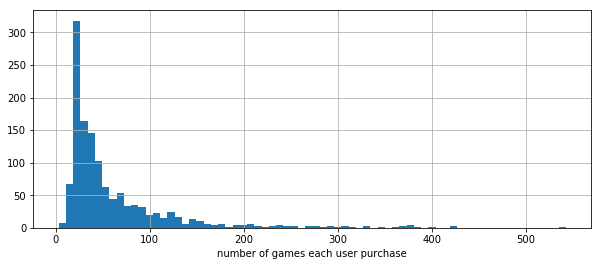
\includegraphics[width=\textwidth]{./results/user_play_game.png}
 \caption{Steam平台游戏购买数据}
 \label{figure:steam}
\end{figure}

接下来就是,将预处理得到的信息分别由WMF和ExpoMF训练。在训练的过程中,利用NDCG@20的标准,检测ExpoMF的训练结果。
\par
实验结果表明,ExpoMF为用户推荐的游戏列表,在测试集的表现更加优秀(三种评判手段 NDCG@20,MAP@20,Reacll@20 下都如此)。也就是说,ExpoMF推断出的用户向量和物品向量更能反映现实世界的情况。图\ref{figure:performance}的左图给出了训练时检测的NDCG@20,其中WMF只汇报了最终结果,作为性能的参照线,对于ExpoMF,则绘制了每次更新后的性能。可以看出在不断地更新物品和用户隐向量之后,推荐列表的质量越来越高,大约10轮迭代后达到稳定状态。


在测试集上的结果汇总如下:
\begin{table}[htbp]\centering
\begin{tabular}{llll}
\hline\hline
Method             & WMF          & ExpoMF      \\
\hline
discription  	  &Weighted MF    & ExpoMF with Per-Item          \\
MAP@20  		  & 0.05069       & \textbf{0.05620}       \\
NDCG@20           & 0.058667      & \textbf{0.06196}               \\
Recall@20         & 0.20025       & \textbf{0.20135}              \\

\hline
\end{tabular}
\caption{Test scores in Steam}\label{tab:performance_steam}
\end{table}

\par
这个结果是在我们的预期之中的,ExpoMF之所以能取得更好的效果,一个是因为它把原始数据的生成看做了一个混合模型更能真实的反映现实状况,另一个是面对0-1型的数据,WMF本身的优势无法完全发挥出来(当你面对的完全是0和1的时候,你很难分辨该对哪些1数据做区分或对哪些0数据更有信心)。



\begin{figure}[t]
 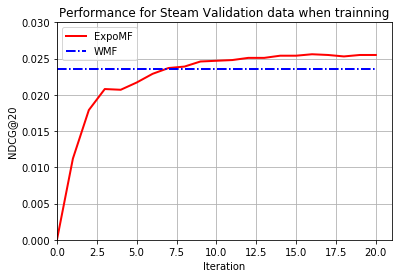
\includegraphics[width=0.5\textwidth]{./results/performance_steam.png}
 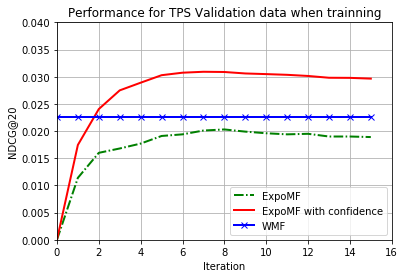
\includegraphics[width=0.5\textwidth]{./results/performance_tps.png}
 \caption{ExpoMF的训练表现}
 \label{figure:performance}
\end{figure}

\section{在TPS数据上测试ExpoMF with confidence}

为了验证ExpoMF在面对非0-1型的数据的时候的性能。我测试了ExpoMF在TPS数据集合上的表现。TPS是一份记录了“用户-音乐”点击次数的数据,经过预处理之后得到400个用户和1013首歌曲。
\par
这份数据和之前的游戏购买记录的不同在于,这份数据中包含了点击的次数,因此传统的WMF方法可以借助这个信息估计出对每个数据的信息。实验结果也表明,直接的ExpoMF的表现会不如WMF。因此,考虑把原始信息中的点击次数借助信心函数,加入进去,即用ExpoMF with confidence。

图\ref{figure:performance}的右图给出了训练时检测的NDCG@20。其中ExpoMF无论是在Validation Set上还是在Test Set上的表现都不如WMF,这是因为两个模型接受的数据含有的信息量不同,直接的ExpoMF二值化了代表“点击次数”的信息,WMF则将这部分信息作为“信心值”,当做了回归的系数,直接的ExpoMF性能不如WMF是可以理解的。
\par
\par
进一步,ExpoMF with confidence也利用了原本代表“点击次数”的信息,把这部分信息用于推断先验估计$\mu_{ui}$,从实验结果看,大大地提高了ExpoMF的性能。这是因为有了原始“点击次数”的信息,能够更加准确的估计推断先验估计$\mu_{ui}$

在测试集上的结果汇总如下:
\begin{table}[htbp]\centering
\begin{tabular}{llll}
\hline\hline
Method             & WMF          & ExpoMF     					 &ExpoMF with confidence\\
\hline
discription  	  &Weighted MF    & with Per-Item Update         &  with Confidnce-Per-Item Update\\
MAP@20  		  & 0.05195       & 0.04139       	    &   \textbf{0.07626}\\
NDCG@20           & 0.05949       & 0.05038             &   \textbf{0.07583}\\
Recall@20         & 0.22503       & 0.20803             &   \textbf{0.24094}\\
\hline
\end{tabular}
\caption{Test scores in TPS}\label{tab:performance_tps}
\end{table}

\section{在Movielens数据上测试ExpoMF with covariates}

ExpoMF中推断先验估计$\mu_{ui}$的另一种思路是,引入外部的“主题信息”,比如地理位置的分类信息,来自文本的信息,或者基于内容的信息。

在Movielens数据集上,我根据原数据集中的电影的分类标签,生成$\psi_u$。Movielens把电影打上分类标签:Action,Adventure,Animation,Children's,Comedy,Crime,Drama等18个分类标签。一个电影可能同时有多个标签,从中可以做分类,或者直接根据这些标签生成向量并规范化,总之,每个电影对应一个分类向量$\psi_u$。

同时作为对比,我同时实验了在不引入外部的基于内容的分类信息的情况下的ExpoMF以及WMF。实验的测试集上的结果如下:
\begin{table}[htbp]\centering
\begin{tabular}{llll}
\hline\hline
Method             & WMF          & ExpoMF     					 &ExpoMF with content\\
\hline
discription  	  &Weighted MF    & with Per-Item Update         &  with Exposure covaviates Update\\
MAP@20  		  & 0.13116       & 0.13427      	    &   \textbf{0.13441}\\
NDCG@20           & 0.14797       & 0.14925             &   \textbf{0.14942}\\
Recall@20         & 0.13138       & 0.13630             &   \textbf{0.13637}\\
\hline
\end{tabular}
\caption{Test scores in Movielens}\label{tab:performance_movie}
\end{table}

\par
可以看出的是,虽然ExpoMF with content的效果相对于ExpoMF最终好一点,但是其实好的非常有限,从推荐效果来说没有非常明显的提升。但是,ExpoMF相对传统WMF还是要好一些的。

\begin{figure}[h]
 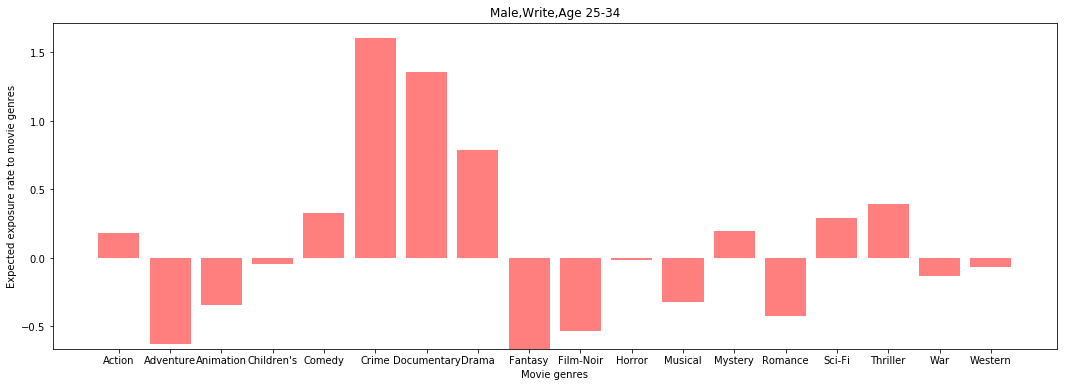
\includegraphics[width=\textwidth]{./results/writer.png}
 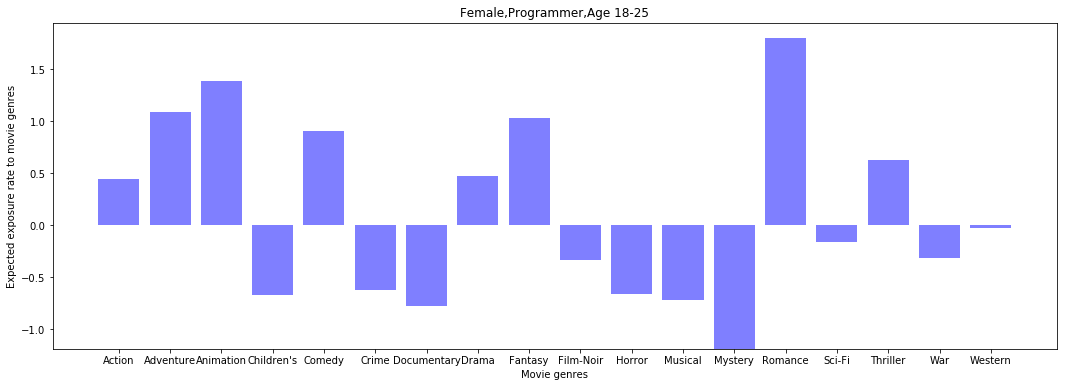
\includegraphics[width=\textwidth]{./results/programmer.png}
 \caption{两个用户对各种类型的电影的暴露比例}
 \label{figure:ExposureRate}
\end{figure}
\par
从挖掘用户的信息的角度来说ExpoMF with content有独到的优势。
\par
首先,ExpoMF with content学习到了用户$u$对各个分类信息的暴露时间的比例$\psi_u$,这个信息可以反映用户平常会花时间在哪些分类的内容上。这是一个有价值的信息,电子商务公司可以从中了解到用户平常会花精力在什么内容的东西上,从而更好的推销商品、合理的展示广告。电子书、电影、音乐或电视剧的公司可以了解用户平常喜欢花时间在什么类型的书上,含有什么元素的电影上,什么风格的音乐上。
\par
针对Movielens数据,我随机抽取了两个用户,分析他们平常会花时间具有哪些特质的电影上。
\par
第一个用户是,男性作家,年龄在25-34岁,模型学习到的他最经常花时间在犯罪片、记录片以及戏剧上,直观看上去的确符合作家的气质,可以参照\ref{figure:ExposureRate}的上面的图。
\par
第二个用户是,女性程序员,年龄在18-25岁,模型学习到的是她经常花时间在浪漫爱情片、动画片和冒险片上,爱看动画片似乎的确是单纯的程序员的特质,而爱看浪漫的爱情片可能可以归结于其女性的属性吧,具体可以参照\ref{figure:ExposureRate}的下面的图。


\par
另外一个ExpoMF with content学习到的有价值的信息在于,模型学习到了一个所有用户的对于不同物品的暴露与否的先验估计$\mu_{ui}$。由于$E[z_{ui}]=\mu_{ui}$,所以借助这个$\mu_{ui}$,我们可以估计一个物品是否已经被用户看到了,我认为这可以帮助营销人员或者广告人员进行精准的促销。借助这个信息,可以进行“向没有注意到某物品的人”营销。
\par
或者更加一般的,利用模型学习到的$\hat{z}_{ui}=E[z_{ui}|\theta_u,\beta_i,y_{ui}]$来估计一个物品是否被用户看到了。
\begin{figure}[h]
 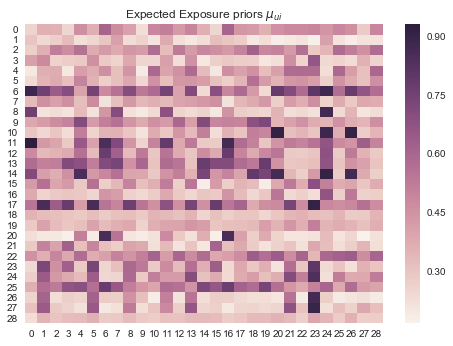
\includegraphics[width=\textwidth]{./results/heatmap.png}
 \caption{估计物品是否被用户看到了,颜色越深,代表越有可能已经被看到}
 \label{figure:heatmap}
\end{figure}

\chapter{结论}
在本论文中,我对最近新提出的一种处理隐式反馈数据的协同过滤方法\cite{EXPOMF}——ExpoMF做了研究,介绍了协同过滤的历史、目前主流的方法以及之前的方法与ExpoMF的区别和联系。同时,针对“点击次数、观看时长”之类的反映“用户行为强烈程度”的原始信息的隐式反馈数据,在ExpoMF的框架下,提出了一种新的模型。
\par
在实验性的探索中,我把ExpoMF实验在三个数据集上:TPS音乐点击数据,Steam游戏购买数据与Movielens电影观看数据上。验证了ExpoMF的性能,并与主流的WMF方法做比较,实验结果证明在各种评价标准下,ExpoMF的确能为用户生成更加优质的推荐列表。



\chapter*{\heiti 致谢}

我要感谢我的母亲,从小到大教我做人的道理,永远的给我鼓励,教会我坚强和勇敢。我要感谢我的奶奶,是从小你抚养我,在每个我长大的瞬间,都是你的身影。现在我即将从复旦数学学院本科毕业了,这篇毕业论文不敢说写的好,但是这是你们从小看着长大的我,认真研究的结果,独立探索的结果,从头到尾脚踏实地实现的结果,献给你们俩。希望以后也能成为你们的骄傲。

\par
其次,感谢在完成这篇论文的时候帮助指导我的张淑芹老师。感谢素昧蒙面的复旦学长、ExpoMF的原作者Dawen Liang,你优秀的论文和代码风格在我完成这篇毕业设计的时候深深的影响了我,以你为榜样。




 \footnotesize
\begin{thebibliography}{99}
\bibitem{WMF} Yifan Hu, Yehuda Koren, and Chris Volinsky, “Collaborative Filtering for Implicit Feedback” , 2008 Eighth IEEE International Conference on Data Mining,2008
\bibitem{EXPOMF} Dawen Liang, Laurent Charlin, James McInerney, David M. Blei, “Modeling User Exposure in Recommendation” ,International Conference on World Wide Web , 2016

\bibitem{MF} Y. Koren, R. Bell, and C. Volinsky. “Matrix factorization techniques for recommender systems.”, Computer, 42(8): 30–37, Aug. 2009. ISSN 0018-9162, 2009

\bibitem{PMF} A. Mnih and R. Salakhutdinov. “Probabilistic matrix factorization.”, In Advances in Neural Information Pro- cessing Systems, pages 1257–1264, 2007
\bibitem{BLOG} S.Funk,“NetflixUpdate:TryThisatHome”,http://sifter.org/~simon/journal/20061211.html ,2006

\bibitem{MSD} T. Bertin-Mahieux, D. P. W. Ellis, B. Whitman, and P. Lamere. The million song dataset. In Proceedings of the 12th International Society for Music Information Retrieval Conference, pages 591–596, 2011.

\bibitem{MLS}F. Maxwell Harper and Joseph A. Konstan. 2015. The MovieLens Datasets: History
and Context. ACM Transactions on Interactive Intelligent Systems (TiiS) 5, 4,
Article 19 (December 2015), 19 pages. DOI=http://dx.doi.org/10.1145/2827872

\end{thebibliography}



%\bibliographystyle{plain}
%\bibliography{../ml}
\end{document}
